\documentclass[tikz,border=3pt]{standalone}
\usepackage{xcolor}
\usetikzlibrary{arrows.meta,decorations.pathmorphing,positioning}
\definecolor{signalblue}{HTML}{2563EB}
\definecolor{alertred}{HTML}{DC2626}
\definecolor{panelgray}{HTML}{E2E8F0}
\begin{document}
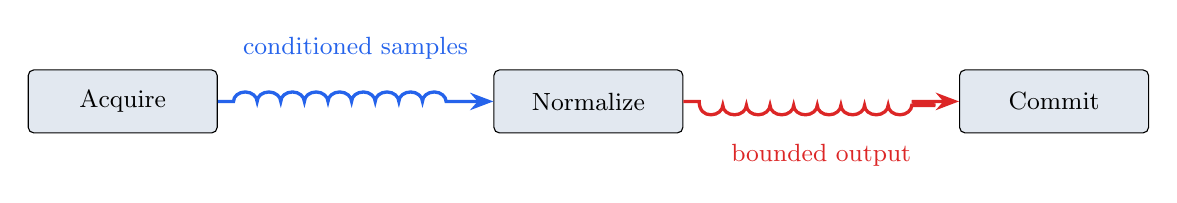
\begin{tikzpicture}[
  >=Stealth,
  process/.style={draw,rounded corners=2pt,minimum width=2.4cm,minimum height=8mm,fill=panelgray},
  every node/.style={font=\small}
]
  \node[process] (input) {Acquire};
  \node[process,right=3.5cm of input] (shape) {Normalize};
  \node[process,right=3.5cm of shape] (output) {Commit};
  \draw[signalblue,very thick,-Stealth,decorate,
    decoration={bumps,segment length=6mm,amplitude=1.2mm,pre length=2mm,post length=3mm}]
    (input) -- node[above=4mm]{conditioned samples} (shape);
  \draw[alertred,very thick,-Stealth,decorate,
    decoration={bumps,segment length=6mm,amplitude=1.2mm,mirror,raise=.5mm,pre length=2mm,post length=3mm}]
    (shape) -- node[below=4mm]{bounded output} (output);
\end{tikzpicture}
\end{document}
